\title{Singularity Software\\Milestone 2}
\date{\today}

\documentclass[12pt]{article}
\usepackage[a4paper]{geometry}
\usepackage{makeidx}
\usepackage[acronym]{glossaries}
\usepackage{pdflscape}
\usepackage{amsmath}
\usepackage{graphicx}
\usepackage[final]{pdfpages}
% \usepackage{hyperref} % Makes links from ToC

\geometry{top=1.0in, bottom=1.0in, left=1.0in, right=1.0in} % Sets the margins

\setlength{\parindent}{0pt} % Fixes the paragraph spacing problem

% This is all for formatting and making the Table of Contents according to 
% spec. Don't play with it.
\makeatletter
\renewcommand\l@section[2]{%
  \ifnum \c@tocdepth >\z@
    \addpenalty\@secpenalty
    \addvspace{1.0em \@plus\p@}%
    \setlength\@tempdima{1.5em}%
    \begingroup
      \parindent \z@ \rightskip \@pnumwidth
      \parfillskip -\@pnumwidth
      \leavevmode \bfseries
      \advance\leftskip\@tempdima
      \hskip -\leftskip
      #1\nobreak\ 
      \leaders\hbox{$\m@th\mkern \@dotsep mu\hbox{.}\mkern \@dotsep mu$}
     \hfil \nobreak\hb@xt@\@pnumwidth{\hss #2}\par
    \endgroup
  \fi}
\makeatother

\makeindex

% Construct the glossary here
% Use the template below, then where the word appears (in the case below, computer), replace computer with \gls{computer}
\makeglossaries

\newglossaryentry{Sifteo Cubes}
{
  name={Sifteo Cubes},
  description={are small machines capable of loading programs and interacting with one another as well as responding to predefined movements}
}

\newglossaryentry{Object-Oriented Programming}
{
  name={Object-Oriented Programming},
  description={is a programming paradigm using objects to design applications}
}

\newglossaryentry{Windows}
{
  name={Windows},
  description={is a series of operating systems developed by Microsoft}
}

\newglossaryentry{Mac}
{
  name={Mac},
  description={is a series of lines of personal computers developed by Apple}
}

\newglossaryentry{Linux}
{
  name={Linux},
  description={is a Unix-based operating system based on free and open source software}
}

\newglossaryentry{cross-platform support}
{
  name={cross-platform support},
  description={is an attribute given to software implemented and operable on multiple computer platforms}
}

\newacronym{API}{API}{\glsadd{API}{Application Programming Interface}}

\newglossaryentry{APIg}
{
  name={Application Programming Interface},
  description={is an interface implemented by a software program that enables it to interact with other software}
}


\newglossaryentry{open source}
{
  name={open source},
  description={is an attribute given to software for which the source code is freely available}
}

\newacronym{IDE}{IDE}{\glsadd{IDE}{Integrated Development Environment}}

\newglossaryentry{IDEa}
{
  name={Integrated Development Environment},
  description={is software that provides a comprehensive work environment for computer programmers and software developers}
}


\newacronym{GUI}{GUI}{\glsadd{GUI}{Graphical User Interface}}

\newglossaryentry{GUIa}
{
  name={Graphical User Interface},
  description={is a visual way of allowing the User to interace with a computer program}
}

\newglossaryentry{version control}
{
  name={version control},
  description={is the management of documents and programs for a project over many versions in a well-organized manner}
}

\newglossaryentry{issue tracking system}
{
  name={issue tracking system},
  description={is a piece of software used to maintain a list of issues as generated during a project}
}

\renewcommand*\arraystretch{1.5}

\begin{document}
\vspace*{\fill}
        \begin{center}
                \LARGE{Singularity Software} \\
                \LARGE{\textit{Milestone 2}} \\
                \vspace{.15in}
                \large{\today} \\
                \vspace{4in}
                By signing below, I approve the contents of the following document. \\
                \begin{table}[h]
                        \begin{tabular}{p{2in} p{5.5in}}
%                \begin{align*}
                        & \\
                        Alex Mullans & \line(1,0){285} \\ & \\
                        Ruben Rodriguez & \line(1,0){285} \\ & \\
                        Ethan Veatch & \line(1,0){285} \\ & \\
                        Kurtis Zimmerman & \line(1,0){285}
                        \end{tabular}
                \end{table}
%                \end{align*}
        \end{center}
\vspace*{\fill}
\thispagestyle{empty}

\clearpage

\tableofcontents

\clearpage
        
\section{Executive Summary}
This document is the second in a series of milestone documents that will accompany the planning of the Siftables\index{Siftables} Emulator\index{emulator}. The Emulator\index{emulator} project is a first of its kind application that will allow developers of Sifteo applications to test the features of the Cubes in a virtual programming environment. Currently, the only way to test apps developed for the Sifteo Cubes\index{Sifteo Cubes} platform is with the physical Cubes; this project will eliminate that need and serve as a demo for the possibilities of the Sifteo platform.\\\\
This milestone elaborates the functions and features of the the Siftables\index{Siftables} Emulator\index{emulator} project. It first gives a brief background of the project before moving on to describe features with use cases and declarative statements, where appropriate. It also maps all covered use cases to their relevant features. Finally, it presents mockups of the Emulator's\index{emulator} design for consideration and to solicit client feedback.  Future milestones will present plans for change control, coding standardization, and testing. Finally, design and usability reports will make up the core of milestones near the end of the quarter as the software stabilizes.


\section{Introduction}
Developers of applications for the \gls{Sifteo Cubes}\index{Sifteo} currently must test programs they create for the platform on the Cubes themselves.  With a full release of the Cubes and corresponding \gls{API}\index{API}\glsadd{APIg} still pending, developers unable to join the Sifteo Early Access program are left without a software-based interface within which to productively develop Sifteo programs. As such, Singularity Software will provide, in the form of the Siftables Emulator\index{emulator}, a software-based emulator\index{emulator} for the Sifteo Cubes that will allow any developer to try programming in the unqiue environment provided by the Cubes.\\\\
Milestone 2 lays the foundation of the Siftables Emulator specification based on the requirements gathered in Milestone 1. It will be supplemented by the specification and prototypes in Milestone 3. Milestone 4 will rely on these early milestones as they define a change control plan and test cases, and Milestone 5 will elaborate the usability guidelines and interface design that implement the features and use cases described herein.


\section{Project Background}
The Siftables Emulator is being developed by Singularity Software as part of the Junior Project sequence of classes at Rose-Hulman Institute of Technology. When projects were solicited for the sequence, clients Tim Ekl and Eric Stokes (both Rose-Hulman alumni) submitted a request for an emulator\index{emulator} for Sifteo Cubes\index{Sifteo Cubes}, a new platform intended for ``intelligent play." After Singularity was chosen for the project, we met with Mr. Ekl to determine the three primary features of the Emulator: a Workspace where 1-6 Cubes could mimic the manipulations possible with physical Cubes, an \gls{API} to program those virtual Cubes, and a set of example games designed to show off the first two features. Singularity's Emulator\index{emulator} will be the first program of its kind on the market for Sifteo Cubes. \\

A full feature listing and description can be found in Appendix A.

\clearpage

\section{Use Cases}

  \subsection{Load program}

    \begin{description}
      \item[Name:] Load program
      \item[Description:] The User selects the program file to be loaded and run by the emulator\index{emulator}.
      \item[Actors:] User
      \item[Basic flow:] \hfill 
        \begin{enumerate}
	  \item{The User presses the ``Load a program" button.}
	  \item{The User selects a *.siftem file in the file dialog.}
	  \item{The User presses ``Open" button.}
	  \item{The emulator loads the selected program on the Cubes in the emulator.}
        \end{enumerate}
      \item[Alternate flows:] \hfill \\
	When the User opens an incompatible file (i.e. any file without the .siftem extension),
        \begin{enumerate}
			\item{An error dialog is presented to the User with the message: "The selected file is not a .siftem emulator file and cannot be loaded."}
			\item{The use case terminates and no program is loaded.}
        \end{enumerate}
	When the User opens a corrupt or otherwise unloadable file,
        \begin{enumerate}
			\item{An error dialog is presented to the User with the message: "The selected file is corrupt and cannot be loaded."}
			\item{The use case terminates and no program is loaded.}
        \end{enumerate}
	When the User presses the ``Cancel" button:
        \begin{enumerate}
			\item{The use case terminates and no program is loaded.}
        \end{enumerate}
	When the User is already running a program,
		\begin{enumerate}
			\item{A warning dialog is presented to the User with the message: "Loading this program will clear all data from the previous program run. Proceed?"}
			\item{If the User presses ``Yes" on the warning dialog, flow returns to Step 2 of the basic flow.}
		\end{enumerate}
	When the User presses ``No" on the warning dialog:
        \begin{enumerate}
          \item{The use case terminates and the program is not reloaded.}
        \end{enumerate}
      \item[Pre-conditions:] \hfill
        \begin{enumerate}
          \item{The emulator is running.}
        \end{enumerate}
      \item[Post-conditions:] \hfill
        \begin{enumerate}
	  \item{The program is loaded or the User cancelled loading.}
        \end{enumerate}
      \item[Special requirements] \hfill
        \begin{enumerate}
          \item{The emulator should indicate that loading the program is in progress.}
          \item{The emulator should indicate when the program is finished loading.}
        \end{enumerate}
    \end{description}
%\newpage
  \subsection{Reload program}

    \begin{description}
      \item[Name:] Reload program
      \item[Description:] The User reloads the program currently running in the emulator.
      \item[Actors:] User
      \item[Basic flow:] \hfill
        \begin{enumerate}
			\item{A warning dialog is presented to the User with the message: "Reloading this program will clear all data from the previous program run. Proceed?"}
			\item{If the User presses ``Yes" on the warning dialog, the Emulator loads the program onto the Cubes in the emulator.}
        \end{enumerate}
      \item[Alternate flows:] \hfill \\
	When the User presses ``No" on warning dialog:
        \begin{enumerate}
          \item{The use case terminates and the program is not reloaded.}
        \end{enumerate}
      \item[Pre-conditions:] \hfill
        \begin{enumerate}
	  \item{A program is loaded in the emulator.}
        \end{enumerate}
      \item[Post-conditions:] \hfill
        \begin{enumerate}
	  \item{The program is reloaded or the current program state remains on the Cubes.}
        \end{enumerate}
      \item[Special requirements:] \hfill
        \begin{enumerate}
          \item{The emulator should indicate that loading the program is in progress.}
	  \item{The emulator should indicate when the program is finished loading.}
        \end{enumerate}
    \end{description}

  \subsection{Zoom screen}

    \begin{description}
      \item[Name:] Zoom screen
      \item[Description:] The User zooms the Workspace to the desired level.
      \item[Actors:] User
      \item[Basic flow:] \hfill
        \begin{enumerate}
	  \item{The User adjusts the zoom slider.}
	  \item{The Emulator magnifies the Cubes in the emulator according to the zoom level.}
        \end{enumerate}
      \item[Alternate flows:] \hfill \\
	None
      \item[Pre-conditions:] \hfill
        \begin{enumerate}
          \item{The emulator is running.}
        \end{enumerate}
      \item[Post-conditions:] \hfill
        \begin{enumerate}
	  \item{The program running at the beginning of this use case, if any, is still running.}
        \end{enumerate}
	  \item[Special requirements:] \hfill
        \begin{enumerate}
		\item{The zoom slider moves in discrete increments. The lowest (and default) level shows the whole workspace and the highest level shows one Cube with the edges of the surrounding Cubes visible for context.}
		\end{enumerate}
    \end{description}	

  \subsection{Add/remove Cubes}

    \begin{description}
      \item[Name:] Add/remove Cubes
      \item[Description:] The User adjusts the number of Cubes present in the emulator.
      \item[Actors:] User
      \item[Basic flow:] \hfill
        \begin{enumerate}
	  \item{The User drags the ``Number of Cubes" slider or uses the up/down arrows on the spinbox to increment or decrement the number of available Cubes by one.}
	  \item{The emulator adds/removes Cubes in emulator and resets its Workspace.}
	  \item{If Cubes are to be removed, the emulator starts with the bottom right-most of the Cubes (at their current positions) and works left. If more Cubes are to be removed after the second row is depleted, the emulator again starts at the bottom right-most of the remaining Cubes.}
        \end{enumerate}
      \item[Alternate flows:] \hfill \\
	None
      \item[Pre-conditions:] \hfill
        \begin{enumerate}
	  \item{The emulator is running.}
        \end{enumerate}
      \item[Post-conditions:] \hfill
        \begin{enumerate}
	  \item{The number of Cubes has been adjusted to the number specified.}
	  \item{The running program, if any, is terminated.}
        \end{enumerate}
	  \item[Special requirements:] \hfill
        \begin{enumerate}
		\item{The ``Number of Cubes" slider moves in discrete increments. The leftmost level shows one Cube and the rightmost level shows six Cubes.}
		\end{enumerate}
    \end{description}

  \subsection{Snap Cubes to grid}

    \begin{description}
      \item[Name:] Snap to grid
      \item[Description:] The Users pulls the Cubes into a grid orientation.
      \item[Actors:] User
      \item[Basic flow:] \hfill
        \begin{enumerate}
	  \item{The User presses the ``Snap to Grid" button.}
	  \item{The Emulator moves the Cubes to a grid orientation based on their current positions. It will maintain the Cubes' positions relative to other Cubes while doing so.}
        \end{enumerate}
      \item[Alternate flows:] \hfill \\
	None	
      \item[Pre-conditions:] \hfill
        \begin{enumerate}
	  \item{The emulator is running.}
        \end{enumerate}
      \item[Post-conditions:] \hfill
        \begin{enumerate}
	  \item{The Cubes are arranged in a grid.}
        \end{enumerate}
    \end{description}

  \subsection{Manipulate Cube}

    \begin{description}
      \item[Name:] Manipulate Cube
      \item[Description:] The User manipulates a Cube by clicking the buttons or the Cube itself.
      \item[Actors:] User
      \item[Basic flow:] \hfill
        \begin{enumerate}
	  \item{The User double clicks on a Cube.}
	  \item{The Cube responds as if a screen click occured.}
        \end{enumerate}
      \item[Alternate flows:] \hfill
        \begin{enumerate}
	  \item{The User clicks on one of the buttons superimposed on the Cubes' edges.}
	  \item{The Cube executes the appropriate action (i.e. flips, rotates, or tilts).}
        \end{enumerate}
        \begin{enumerate}
          \item{The User drags a Cube next to another Cube.}
	  \item{Cube communicates (``neighbors") with the Cube(s) it is adjacent to.}
        \end{enumerate}
	  \item{The User ``shakes" a Cube back and forth with the mouse (i.e. he laterally moves the Cube back and forth several times).}
	  \item{The Cube responds as if shaken.}
      \item[Pre-conditions:] \hfill
        \begin{enumerate}
          \item{The emulator is running.}
        \end{enumerate}
      \item[Post-conditions:] \hfill
        \begin{enumerate}
	  \item{If a program is running, the emulator has updated its state based on the Cube's change.}
        \end{enumerate}
    \end{description}
	
  \subsection{Other functional requirements}

	\subsubsection{API}
		The emulator will include an API in order to define a set of rules and specifications via which Cube programs can be created.
	
	\subsubsection{Example games}
		The emulator will include games as examples that demonstrate to the User how the Cubes interact with each other.

%\newpage
\section{Use Case Feature Mapping}
    The feature listing can be found in appendix A, and the use case IDs refer to the use cases specified above.
    \begin{table}[h]
      \begin{tabular}{l | l | l}
        \textbf{Use case ID} &
        \textbf{Use case} &
        \textbf{Feature ID} \\ \hline

        U1 &
        Load program &
        F5 \\

        U2 &
        Reload program &
        F5 \\

        U3 &
        Zoom screen &
        F7 \\

        U4 &
        Add/remove Cubes &
        F3, F4\\

        U5 &
        Snap Cubes to grid &
        F6 \\

        U6 &
        Manipulate Cube &
        F1, F2, F3 \\
		
	OR1 & 
	API &
	F2 \\
		
	OR2 &
	Example games &
	F3 \\

      \end{tabular}
    \end{table}

\section{Work/Data Flow Diagrams}
The following pages contain work/data flow diagrams that elucidate the passage of control and data through the emulator. As there is not much pure data that flows through the emulator system aside from the User's program, Singularity Software has elected to combine the workflow and data flow diagrams.

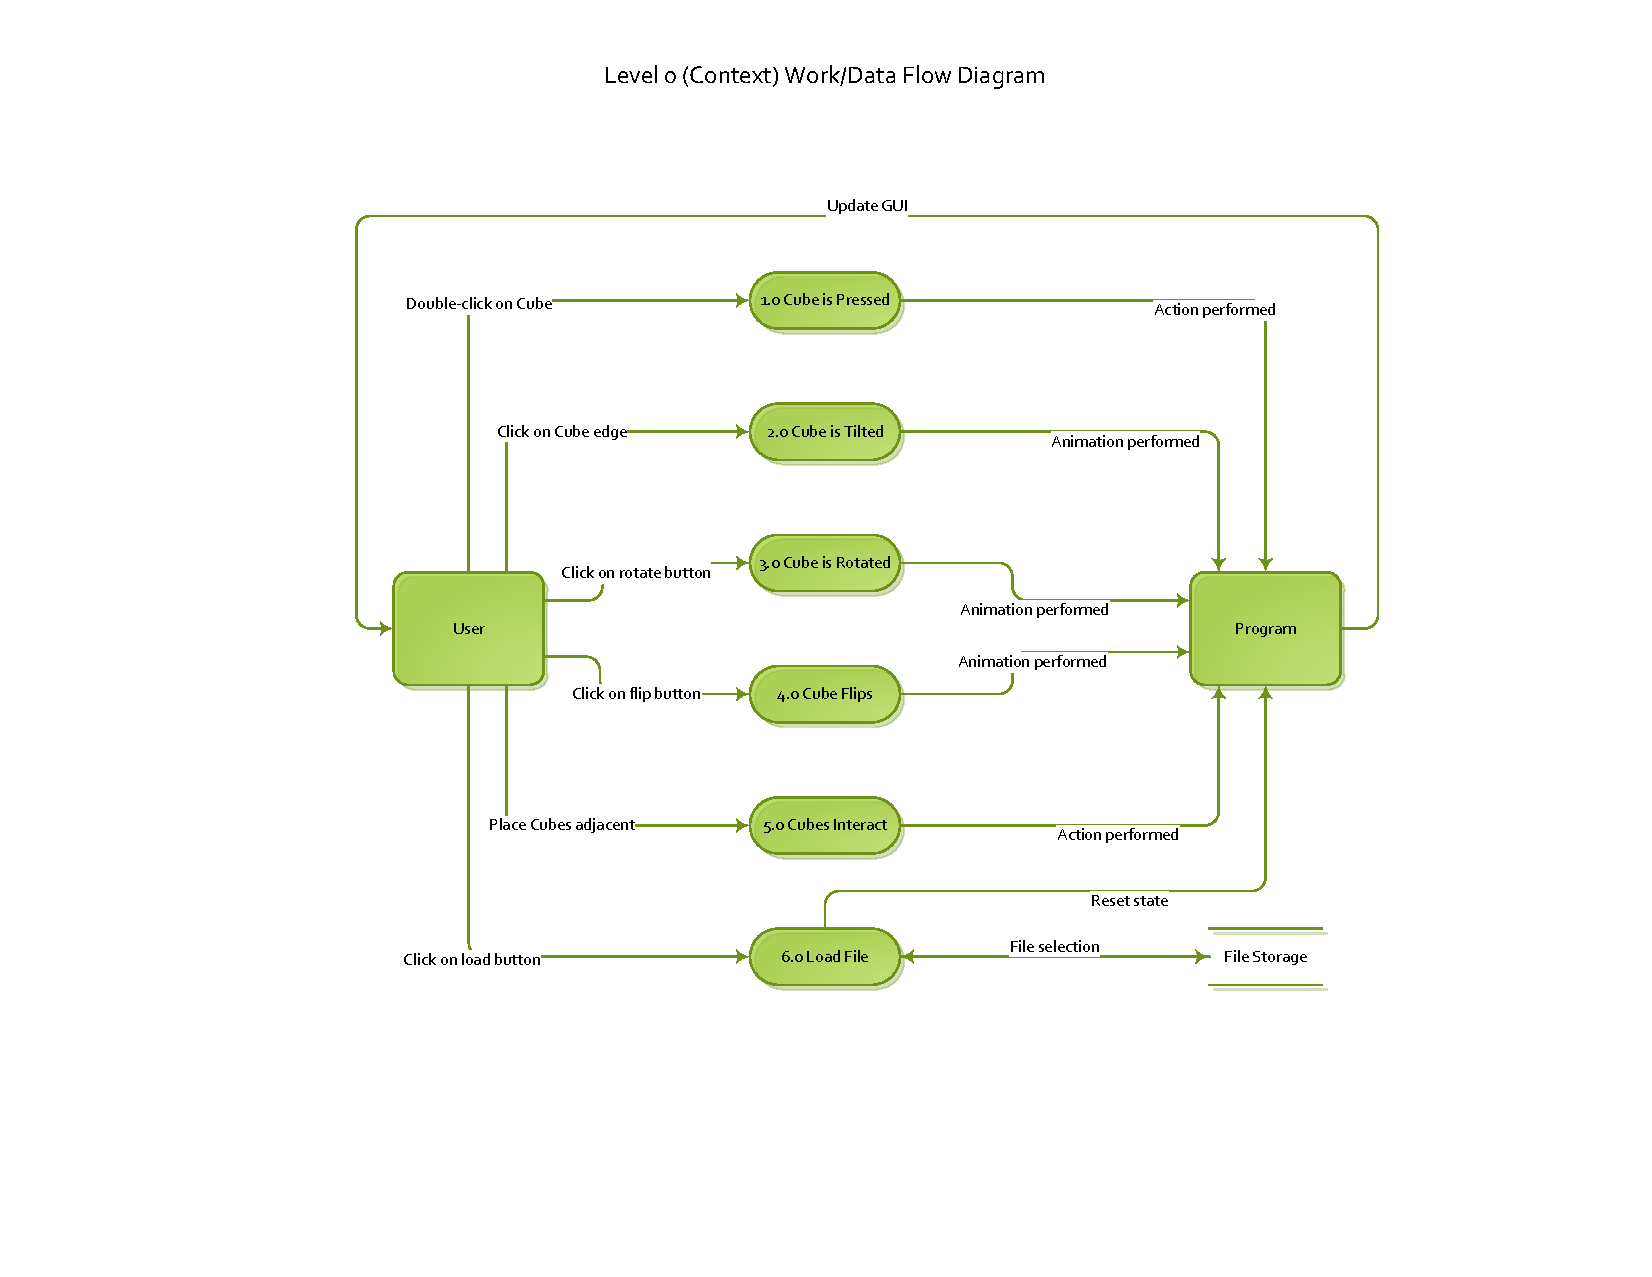
\includepdf[pages={1-7},landscape]{pdfs/dfds.pdf}

\appendix
    \begin{landscape}
    \section{Features}
    \begin{table}[h!]
      \begin{tabular}{p{.25in} | p{2.75in} | p{3in} | p{3in}}
        \textbf{ID} &
        \textbf{Feature} &
        \textbf{Description} &
        %\textbf{Status} &
        %\textbf{Priority} &
        %\textbf{Risk} &
        %\textbf{Stability} &
        \textbf{Reason} 
        %\textbf{Effort}
        \\ \hline

        F1 &
        Individual, virtual Sifteo Cube &
        A virtual representation of a single Sifteo Cube &
        %Approved &
        %Critical &
        %Low &
        %High &
        Replicates physical Sifteo Cube
        %Medium 
        \\ \hline

        F2 &
        Buttons to manipulate each virtual Cube &
        Buttons on the virtual Cube will allow the User to flip and tilt it &
        %Approved &
        %Critical &
        %Medium &
        %High &
        Replaces physical actions where said actions would be impractical with a mouse
        %Medium
        \\ \hline

        F3 &
        Workspace where multiple Cubes can be emulated &
        Multiple Cubes will be displayed on a workspace that replicates the free-form nature of physical Sifteo Cubes\index{Sifteo Cubes} &
        %Approved &
        %Critical &
        %Low &
        %High &
        Replicates multiple Sifteo Cubes\index{Sifteo Cubes} in a natural, free-form environment
        %High
        \\ \hline

        F4 &
        Interactions between Cubes &
        The Cubes present on the workspace will communicate when they are neighbored &
        %Approved &
        %Critical &
        %Low &
        %High &
        Cubes can simulate the interactions possible with physical Cubes
        %High 
        \\ \hline

        F5 &
        Load programs into the Cubes &
        The User will load his own and example programs into the emulator’s\index{emulator} Cubes &
        %Approved &
        %Critical &
        %Medium &
        %High &
        The ability to program programs for the emulator\index{emulator} is dependent on a common interface
        %High
        \\ \hline

        F6 &
        Snap Cubes to invisible grid &
        The Cubes will snap into an invisible grid when a button is clicked &
        %Proposed &
        %Useful &
        %Medium &
        %High &
        Increases productivity by allowing a quick reset if the Cubes are in disarray
        %Low
        \\ \hline

        F7 &
        Zoom Workspace &
        The Workspace will zoom to the level of an individual Cube or the whole space &
        %Proposed &
        %Useful &
        %Low &
        %High &
        Inspecting individual Cubes allows for precise checks of program \glspl{GUI}\index{GUI}\glsadd{GUIa}
        %Low
        \\ \hline

      \end{tabular}
    \end{table}
    \end{landscape}

\clearpage
\addcontentsline{toc}{section}{Glossary}
\printglossaries
\clearpage

\addcontentsline{toc}{section}{References}
\section*{References}

        \begin{enumerate}
                \item{Sifteo Inc. Online: http://www.sifteo.com}
                \item{Tim Ekl.  Client Meeting.  12 September 2011 12:45 p.m.}
        \end{enumerate}

\clearpage

\addcontentsline{toc}{section}{Index}
\printindex

\end{document}
